\documentclass[aps,pra,reprint,superscriptaddress,amsmath,amssymb,longbibliography]{revtex4-2}

\usepackage{graphicx}
\usepackage{xcolor}
\usepackage{booktabs}
\usepackage{bm}
\usepackage[colorlinks=true,linkcolor=blue!60!black,citecolor=blue!60!black,urlcolor=blue!60!black]{hyperref}

% generated by make_paper2.py
\newcommand{\NeNsf}{504}
\newcommand{\NeAB}{504.6}
\newcommand{\NeR}{448.47}
\newcommand{\NeSmax}{1\times10^{-513}}
\newcommand{\NeAbove}{yes}
\newcommand{\MgNsf}{103}
\newcommand{\MgAB}{103.7}
\newcommand{\MgR}{174.78}
\newcommand{\MgSmax}{2\times10^{-113}}
\newcommand{\MgAbove}{yes}
\newcommand{\ArNsf}{105}
\newcommand{\ArAB}{105.4}
\newcommand{\ArR}{114.38}
\newcommand{\ArSmax}{2\times10^{-113}}
\newcommand{\ArAbove}{yes}
\newcommand{\CaNsf}{103}
\newcommand{\CaAB}{103.5}
\newcommand{\CaR}{198.84}
\newcommand{\CaSmax}{4\times10^{-113}}
\newcommand{\CaAbove}{yes}
\newcommand{\ZnNsf}{104}
\newcommand{\ZnAB}{105.0}
\newcommand{\ZnR}{162.58}
\newcommand{\ZnSmax}{6\times10^{-113}}
\newcommand{\ZnAbove}{yes}
\newcommand{\KrNsf}{105}
\newcommand{\KrAB}{105.8}
\newcommand{\KrR}{121.44}
\newcommand{\KrSmax}{8\times10^{-114}}
\newcommand{\KrAbove}{yes}
\newcommand{\SrNsf}{103}
\newcommand{\SrAB}{103.9}
\newcommand{\SrR}{208.14}
\newcommand{\SrSmax}{4\times10^{-113}}
\newcommand{\SrAbove}{yes}
\newcommand{\PdNsf}{106}
\newcommand{\PdAB}{106.5}
\newcommand{\PdR}{151.69}
\newcommand{\PdSmax}{1\times10^{-112}}
\newcommand{\PdAbove}{yes}
\newcommand{\CdNsf}{105}
\newcommand{\CdAB}{105.2}
\newcommand{\CdR}{170.84}
\newcommand{\CdSmax}{2\times10^{-112}}
\newcommand{\CdAbove}{yes}
\newcommand{\XeNsf}{105}
\newcommand{\XeAB}{105.9}
\newcommand{\XeR}{130.03}
\newcommand{\XeSmax}{2\times10^{-112}}
\newcommand{\XeAbove}{yes}
\newcommand{\KrKappaOne}{32.25}
\newcommand{\KrGrowth}{1701}
\newcommand{\KrPots}{47}
\newcommand{\KrM}{110}
\newcommand{\KrSeg}{67}
\newcommand{\KrUnknowns}{7323}
\newcommand{\KrNodes}{0.45, 1.26}
\newcommand{\KrOneSGap}{129}
\newcommand{\KrOneSAtTen}{-11}
\newcommand{\KrOneSOwnAtTen}{-140}
\newcommand{\HeavyMin}{103}
\newcommand{\HeavyMax}{106}
\newcommand{\CaTimeA}{7}
\newcommand{\KrTimeA}{37}
\newcommand{\XeTimeA}{3.9}
\newcommand{\CertMinH}{0.2}
\newcommand{\CertMaxH}{2.1}
\newcommand{\NeEsplit}{\mathord{-}128.547\,098\,109\,382\,042\,376\,475\\ &\hphantom{-128.}781\,341\,993\,899\,003\,173\,076\\ &\hphantom{-128.}242\,596\,929\,050\,687}
\newcommand{\NeNsfAll}{504}
\newcommand{\NeCertTime}{17}
\newcommand{\NeTimeA}{26}
\newcommand{\NeTimeB}{41}
\newcommand{\NAtomsDone}{10}
\newcommand{\CinalAgree}{Ne, Mg, Ar, Ca, Zn, Kr, Sr, Pd, Cd, Xe}
\newcommand{\NCinalAgree}{10}
\newcommand{\NeMaxOrder}{626}

\newcommand{\eh}{E_\mathrm{h}}
\newcommand{\EHF}{E_\mathrm{HF}}

\begin{document}

\title{FROST II: certified Hartree--Fock limits of the closed-shell atoms from neon to xenon}

\author{Adam L. Baskerville}
\email{adamlukebaskerville@gmail.com}
\noaffiliation

\begin{abstract}
We extend FROST (Fock radial orbital shooting with Taylor series) from atoms whose occupied orbitals are all $s$ orbitals to closed-shell atoms with $p$ and $d$ shells, and report rigorous upper bounds on the Hartree--Fock (HF) energies of the closed-shell atoms from neon to xenon. Their leading digits are correct to \NeNsf\ significant figures for neon, \MgNsf\ for magnesium, \ArNsf\ for argon and \HeavyMin--\HeavyMax\ for the heavier atoms, against previous records of 30 and 25. Three changes to the method make this possible. First, exchange with multipoles $k\ge1$ gives every canonical orbital the exponential tail of the outermost one, so all orbitals must share one wall; this also makes them exactly orthogonal. Second, over that common wall the inner shells are extremely stiff: the growing mode of the krypton $1s$ orbital rises by $10^{\KrGrowth}$. The equations are therefore solved by multiple shooting, with Taylor-series segments short enough that no mode grows by more than $10^g$, coupled by continuity conditions and solved by Newton's method with a sparse LU factorization, so that the working precision grows with the target accuracy rather than with the stiffness. Third, a homotopy in the electron--electron coupling, from hydrogenic orbitals, supplies a starting point that converges to the ground state. The exact-rational certificate carries over to any angular momentum. Writing each radial function as $P=r^{l+1}f$ with $f$ piecewise polynomial, the triangle rule $k\le l_a+l_b$ cancels the factor $r^{-k-1}$ of every multipole, so all overlap, one-electron and Slater integrals are exact rationals. All 25 published digits of the quadruple-precision energies of Cinal are reproduced, as are his positions of the exchange-induced nodes of inner orbitals, which we locate to about 100 significant figures.
\end{abstract}

\maketitle

%=====================================================================================
\section{Introduction}
%=====================================================================================

In a previous paper~\cite{FROST1} (paper I) we obtained the Hartree--Fock (HF) limits of helium and beryllium to 503 and 501 significant figures, without a basis set. The radial HF equations were integrated by arbitrary-order Taylor series in arbitrary-precision arithmetic, the orbital energies were fixed by shooting to a hard wall, and an independent program turned the resulting piecewise-polynomial orbitals into an exact rational upper bound on the energy. Paper I treated only atoms whose occupied orbitals are all $s$ orbitals. Most closed-shell atoms are not of this kind.

The HF limits of heavier atoms have been computed by many numerical methods: finite differences~\cite{FroeseFischer1977,Kobus2013,KobusLehtola2025}, B-splines~\cite{Saito2009}, finite elements~\cite{Lehtola2019} and Slater-type expansions~\cite{Clementi1974}. In double precision these give 10--14 significant figures. Cinal's pseudospectral method in quadruple precision reached 25 figures for all 18 closed-(sub)shell atoms from helium to nobelium~\cite{Cinal2020}, and Yamamoto and Hatano have recently reported 30-figure energies for atoms up to the third period with Laguerre-type $\Lambda$ functions, also in quadruple precision~\cite{Yamamoto2026}. No HF energy of a closed-shell atom beyond beryllium has been known to more than 30 figures.

Three things change when the occupied orbitals include $p$ and $d$ shells.
\begin{itemize}
\item \textbf{Multipoles.} Exchange between orbitals of different angular momentum involves the multipoles $r_<^k/r_>^{k+1}$ with $k\ge1$. Each needs its own pair potential, and krypton already has \KrPots\ of them.
\item \textbf{Tails.} A nonvanishing multipole moment couples an inner orbital to the tail of the outermost one. As Handy, Marron and Silverstone showed~\cite{HMS1969}, every canonical HF orbital then decays with the exponent of the highest occupied orbital. In paper I each beryllium orbital had its own wall; with $p$ and $d$ shells that cuts off the inner orbitals' tails, and one common wall is required (Sec.~\ref{sec:wall}).
\item \textbf{Stiffness.} With a common wall, the inner orbitals' growing modes must be controlled over the whole range. For krypton, $e^{\kappa_{1s}R}$ with $\kappa_{1s}=\KrKappaOne$ and $R=\KrR$~bohr is $10^{\KrGrowth}$, far beyond any working precision. Paper I's nested single shooting cannot cope with this.
\end{itemize}
The contributions of this paper are:
\begin{enumerate}
\item A formulation in which every orbital and every multipole potential obeys an ODE of the same form, $ru''+2(L+1)u'=g$, so that a single Frobenius--Taylor recurrence serves all of them, with one common wall (Sec.~\ref{sec:formulation}).
\item Multiple shooting with Taylor segments, a homotopy in the electron--electron coupling, and wall continuation. Together they give the HF limit to any number of digits with working precision of about the target plus a stiffness margin that does not depend on $\kappa_{1s}/\kappa$ (Sec.~\ref{sec:numerics}).
\item The exact certificate for any angular momentum (Sec.~\ref{sec:certify}).
\item Certified HF limits for Ne, Mg, Ar, Ca, Zn, Kr, Sr, Pd, Cd and Xe, which agree with all published digits~\cite{Cinal2020}, and the exchange-induced nodes of their inner orbitals to about 100 digits (Sec.~\ref{sec:results}).
\end{enumerate}

%=====================================================================================
\section{Formulation}\label{sec:formulation}
%=====================================================================================

This section puts the HF equations into a form that a single numerical tool can handle: we first choose variables in which every equation has the same shape (Sec.~\ref{sec:equations}), then show why all orbitals must share one wall (Sec.~\ref{sec:wall}), and finally write the energy so that it can later be evaluated exactly (Sec.~\ref{sec:energy}).

\subsection{Equations}\label{sec:equations}

Each orbital $a$, with quantum numbers $(n_a,l_a)$, is doubly occupied in all $2l_a+1$ magnetic sublevels, and its normalised radial function $P_a(r)$ behaves as $r^{l_a+1}$ near the nucleus. Dividing out this factor, we work with
\begin{equation}
f_a=P_a/r^{l_a+1},
\end{equation}
which is an ordinary power series at $r=0$. The electrons interact through the multipole potentials
\begin{equation}
Y^k_{ab}(r)=r\int_0^\infty P_a(s)P_b(s)\frac{r_<^k}{r_>^{k+1}}\,ds,
\end{equation}
one for each pair of orbitals and each $k=|l_a-l_b|,|l_a-l_b|+2,\dots,l_a+l_b$, and since these behave as $r^{k+1}$ near the nucleus we likewise work with $y^k_{ab}=Y^k_{ab}/r^{k+1}$. In these variables the canonical closed-shell HF equations are
\begin{align}
rf_a''+2(l_a+1)f_a'={}&2\Big[\Big(r\Big(2\sum_b(2l_b+1)y^0_{bb}-y^0_{aa}\Big) \nonumber\\
&-Z-\varepsilon_ar\Big)f_a \nonumber\\
&-\sum_{(b,k)\ne(a,0)}e^k_{ab}\,r^{k+1+l_b-l_a}\,y^k_{ab}f_b\Big], \label{eq:fock}\\
ry^{k\,\prime\prime}_{ab}+2(k+1)y^{k\,\prime}_{ab}={}&-(2k+1)\,r^{l_a+l_b+1-k}f_af_b, \label{eq:poisson}
\end{align}
with $e^k_{ab}=(2l_b+1)\begin{pmatrix}l_a&k&l_b\\0&0&0\end{pmatrix}^2$. The first term of Eq.~\eqref{eq:fock} is the Coulomb potential of all the electrons less the $k=0$ self-exchange of orbital $a$, the next two are the nucleus and the orbital energy, and the last sum is the remaining exchange. Equation~\eqref{eq:poisson} is Poisson's equation for each multipole. Because $k\ge|l_a-l_b|$, every power of $r$ is a non-negative integer, so no term is singular, and for $s$ orbitals alone the equations reduce to those of paper I.

The point of these variables is that both equations have the same form,
\begin{equation}
ru''+2(L+1)u'=g, \label{eq:form}
\end{equation}
with $L=l_a$ for an orbital and $L=k$ for a potential, so that one Taylor recurrence (Sec.~\ref{sec:taylor}) integrates every unknown. The origin is a regular singular point of Eq.~\eqref{eq:form}, at which the regular solution is fixed by $u(0)$ alone and has slope $u'(0)=g(0)/(2L+2)$. For an orbital this slope is $f_a'(0)=-Zf_a(0)/(l_a+1)$, which is Kato's cusp condition~\cite{Kato1957}, so the cusp is built in exactly.

\subsection{One common wall}\label{sec:wall}

In paper I each orbital had its own wall, placed where that orbital had decayed, but this fails once $p$ or $d$ shells are present because exchange has a long range. Far outside the electron density $Y^k_{ab}(r)\to m^k_{ab}/r^k$, where $m^k_{ab}=\int_0^\infty s^kP_aP_b\,ds$ is the multipole moment of the pair, so the exchange term in the equation for orbital $a$ behaves as $m^k_{ab}r^{-k-1}P_b(r)$, and what happens next depends on $k$.
\begin{itemize}
\item \textbf{$k=0$.} For $a\ne b$ the moment is the overlap of the two orbitals, which vanishes. Exchange then has no long-range part, and each orbital decays at its own rate $e^{-\kappa_ar}$, with $\kappa_a=\sqrt{-2\varepsilon_a}$, as in paper I.
\item \textbf{$k\ge1$.} The moment is generally nonzero, so the tail of $P_b$ drives the equation for $a$, and if $b$ is the outermost orbital its tail decays more slowly than $a$'s own and dominates. Through chains of such couplings every orbital inherits the decay of the highest occupied orbital~\cite{HMS1969,Handler1980,Ishida1992}.
\end{itemize}
Figure~\ref{fig:tails} shows this for krypton: beyond a few bohr every orbital, the $1s$ included, falls off in parallel with the $4p$, so that at $r=10$~bohr the $1s$ is $10^{\KrOneSAtTen}$ of its maximum rather than the $10^{\KrOneSOwnAtTen}$ its own decay would give. A wall placed at the $1s$ orbital's own decay length would therefore cut off a tail that is really there. In neon, moving the $1s$ wall changed the residuals of the other equations at the $10^{-6}$ level, which rules out separate walls at high accuracy.

\begin{figure}[t]
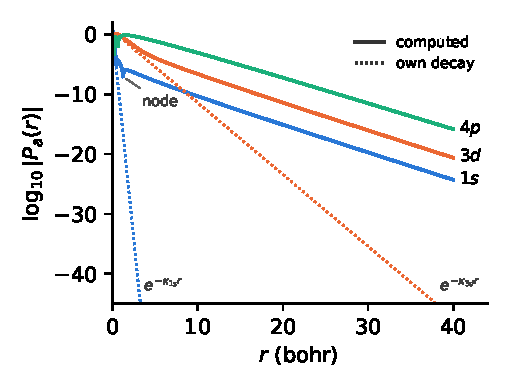
\includegraphics[width=\columnwidth]{fig_tails.pdf}
\caption{Inner orbitals of krypton take on the tail of the outermost one. Solid: computed radial functions $|P_a(r)|$ of the $1s$, $3d$ and $4p$ (run A of Table~\ref{tab:atoms}). Dotted: the decay $e^{-\kappa_ar}$, $\kappa_a=\sqrt{-2\varepsilon_a}$, that the $1s$ and $3d$ would have on their own, drawn from each maximum. Instead both fall off in parallel with the $4p$, because exchange multipoles with $k\ge1$ couple them to its tail (Sec.~\ref{sec:wall}); at $r=10$~bohr the $1s$ lies $10^{\KrOneSGap}$ above its own decay line. The marked dip is one of the two exchange-induced nodes of the $1s$ (Table~\ref{tab:nodes}).}
\label{fig:tails}
\end{figure}

We therefore use one wall $R$ for all orbitals, with the conditions
\begin{gather}
f_a(R)=0,\qquad Ry^0_{aa}(R)=1, \nonumber\\
Ry^{k\,\prime}_{ab}(R)+(2k+1)\,y^k_{ab}(R)=0. \label{eq:bc}
\end{gather}
The first is the wall itself, the second is the normalisation, since $Y^0_{aa}(R)=\int_0^RP_a^2\,dr$, and the third holds exactly outside the density, where $y^k_{ab}\propto r^{-(2k+1)}$.

A common wall brings two further benefits. The orbitals of one symmetry become eigenfunctions of a single self-adjoint Fock operator on $[0,R]$, so they are exactly orthogonal. The walled problem is also the exact HF problem of an atom in a spherical box, whose energy lies above $\EHF$ by an amount that decays as $e^{-2\kappa R}$, with $\kappa$ that of the highest occupied orbital (paper I), and for $D$ digits we therefore take $R=(D+8)\ln10/(2\kappa)$.

\subsection{Energy}\label{sec:energy}

The energy is needed twice, by the solver, which reports it, and by the certificate, which evaluates it exactly for polynomial orbitals (Sec.~\ref{sec:certify}). Because polynomial orbitals are only nearly orthogonal within a symmetry, we use the closed-shell determinant energy, which does not assume orthogonality:
\begin{equation}
\begin{split}
E={}&2\sum_l(2l+1)\sum_{i,j\in l}D_{ij}h_{ij}\\
&+\sum_{l,l'}(2l+1)(2l'+1)\sum_{\substack{i,j\in l\\m,o\in l'}}D_{ij}D_{mo}\\
&\times\Big[2R^0(ij,mo)-\sum_k\begin{pmatrix}l&k&l'\\0&0&0\end{pmatrix}^2R^k(im,jo)\Big].
\end{split}\label{eq:energy}
\end{equation}
Here $D=S^{-1}$ is the inverse overlap matrix within each block of equal $l$, $h_{ij}=T_{ij}+V_{ij}$, and
\begin{equation}
R^k(ij,mo)=\iint P_iP_j(r)P_mP_o(s)\,\frac{r_<^k}{r_>^{k+1}}\,dr\,ds
\end{equation}
are the Slater integrals. Like the $s$-shell energy of paper I, Eq.~\eqref{eq:energy} depends only on the space spanned by the orbitals of each symmetry. In terms of $f$, and after the centrifugal term is integrated by parts, the one-electron integrals are
\begin{equation}
T_{ij}=\frac12\int_0^Rr^{2l+2}f_i'f_j'\,dr,\quad V_{ij}=-Z\int_0^Rr^{2l+1}f_if_j\,dr, \label{eq:onebody}
\end{equation}
because the terms in $r^{2l}f_if_j$ cancel, $-(l+1)(2l+1)+(l+1)^2+l(l+1)=0$, and the boundary terms vanish. The solver evaluates all of these integrals as extra series during the integration.

%=====================================================================================
\section{Numerical method}\label{sec:numerics}
%=====================================================================================

The equations of Sec.~\ref{sec:formulation} form a nonlinear eigenvalue problem in which $n$ orbitals, their potentials and $n$ orbital energies are all coupled. We solve it in four layers. Taylor series integrate the equations step by step (Sec.~\ref{sec:taylor}), and multiple shooting cuts $[0,R]$ into segments so that the growing modes of the inner orbitals never swamp the working precision (Sec.~\ref{sec:shooting}). Newton's method then solves the resulting algebraic equations (Sec.~\ref{sec:newton}), from a starting point supplied by a homotopy and a sequence of growing walls (Sec.~\ref{sec:start}). Appendix~\ref{app:params} lists every parameter.

\subsection{Taylor recurrences}\label{sec:taylor}

Substituting $u=\sum_ku_k(r-r_0)^k$ into Eq.~\eqref{eq:form} gives, about $r_0>0$,
\begin{equation}
u_{k+2}=\frac{g_k-(k+1)(k+2L+2)\,u_{k+1}}{r_0(k+1)(k+2)}, \label{eq:recurrence}
\end{equation}
and about $r_0=0$, $u_{k+1}=g_k/[(k+1)(k+2L+2)]$. The right-hand sides are products of orbitals and potentials, so their coefficients $g_k$ are Cauchy products and a series of order $p$ costs $O(p^2)$ multiplications per product; krypton has 36 pair products $f_af_b$ and 73 exchange products $y^k_{ab}f_b$, about $10^2$ in all. Each step covers a fixed fraction $c$ of the radius of convergence, which the root test estimates from the last coefficients of the orbital series. The truncation error of a step is then about $c^p$, and the order $p$ is chosen to put it below the target accuracy.

One subtlety matters for heavy atoms. The root test sees only the current solution, and because far out every orbital follows the slow common tail, near the wall it would allow a single step across a whole segment. Newton's method, however, also works with each orbital's own fast modes $e^{\pm\kappa_ar}$, which make up the Jacobian columns and the corrections, and at 100 digits such a step resolves them to only 15--20 digits, which is enough to make Newton's method fail. At order $p$ the series of $e^{\kappa r}$ behaves as if its radius of convergence were $p/(e\kappa)$, so we also cap every step at $c\,p/(e\kappa_1)$, with $\kappa_1$ the largest $\kappa_a$; the cap leaves the energies of the light atoms unchanged to every digit.

\subsection{Multiple shooting}\label{sec:shooting}

Over $[0,R]$ the growing mode of the krypton $1s$ rises by $e^{\kappa_{1s}R}=10^{\KrGrowth}$, so shooting from the origin would need that many extra digits. Multiple shooting~\cite{Ascher1995} avoids this by cutting $[0,R]$ into segments, $0=r_0<r_1<\dots<r_J=R$, and integrating each one independently from its own starting state. The unknowns are then the start values $f_a(0)$ and $y^k_{ab}(0)$, the full state $(f_a,f_a',y^k_{ab},y^{k\prime}_{ab})$ at each interior knot and the orbital energies $\varepsilon_a$, while the equations require the state to be continuous at every interior knot and the conditions~\eqref{eq:bc} to hold at $R$. With $n$ orbitals and $n_y$ potentials there are $n_0=n+n_y$ start values, $m=2n_0$ unknowns per knot and $n$ energies; for krypton $n_y=\KrPots$, $m=\KrM$ and $J=\KrSeg$, so the system has \KrUnknowns\ unknowns.

The segments are kept short enough that no growing mode rises, relative to the bulk density $e^{-\kappa r}$, by more than a factor $10^g$ across one. An error in a segment's starting state is then amplified by at most $10^g$, and the linear solve loses at most another $g$ digits, so for $d$ target digits we work with $d+2g+40$ digits. This margin depends on $g$ but not on how stiff the atom is, because a stiffer atom simply needs more segments, and inner orbitals shorten the segments only where they are themselves large (Appendix~\ref{app:params}).

\subsection{Newton's method}\label{sec:newton}

We solve the system by a chord Newton iteration~\cite{Kelley1995}, which keeps one Jacobian and refreshes it only when a step fails to shrink the correction threefold. The Jacobian is formed by forward differences with all columns in one parallel batch, in which a column for a knot state needs only one segment to be integrated again and a column for an $\varepsilon_a$ needs all of them. Its structure is block bidiagonal, with $-I$ coupling each segment to the next knot, plus dense columns for the $\varepsilon_a$, so sparse elimination with row equilibration and partial pivoting keeps the fill inside the band.

Because the chord iteration converges as long as the Jacobian is accurate enough to contract, during the wall continuation (Sec.~\ref{sec:start}) we build and factor it at about $4g+30$ digits, with a matching lower Taylor order. The residuals are always evaluated at full precision, so the converged solution is unchanged, and a cheaper Jacobian that fails is rebuilt at full precision.

\subsection{Starting point and continuation}\label{sec:start}

Newton's method needs a starting point close to the ground state, and the equations for a heavy atom have many other solutions, including ones in which the wall pushes an orbital to positive energy. We therefore reach the ground state in two stages.

The first is a homotopy in the electron--electron interaction: every electron--electron term in Eq.~\eqref{eq:fock} is multiplied by $t$, and the solution is followed from $t=0$, where the hydrogenic orbitals are exact, to $t=1$. Each step in $t$ changes the potentials by a finite amount, which a segment amplifies by $10^g$, so here we keep $g=1$ and a modest target of 10 digits. Meanwhile the wall moves with the orbitals, at $R=\max_a(2n_a+6)/\kappa_a(t)$, where every hydrogenic $r^{n-1}e^{-\kappa r}$ has fallen to about $10^{-3}$ of its peak, so that no orbital is squeezed.

The second stage moves the wall out to its final value, with each step targeting the digits its wall can deliver, $\min(D,2\kappa R/\ln10)+10$. Moving the wall changes the solution only by about $e^{-\kappa R}$ near the old wall, so these steps can afford long segments, with $g$ up to 30. The starting guess on the new knots is the previous solution integrated out to them, continued beyond the old wall with each orbital's own logarithmic derivative and each potential's multipole tail.

\subsection{Implementation}

The orchestration (homotopy, continuation, Newton's method and knot placement) is a few hundred lines of Python with \texttt{gmpy2}, while the numerical work, the integration of a segment and the sparse LU, is done by a small C library on MPFR~\cite{MPFR} and GMP~\cite{GMP}. In the convolutions each product of two MPFR numbers is formed exactly and added to a fixed-point accumulator, and the sum is rounded once~\cite{Kulisch2013}; this is more accurate than a multiply-and-add loop, which rounds $2k+1$ times, and 1.8--2.4 times faster at 170--400 bits. Segments and Jacobian columns are spread over a pool of processes, one per core, and a test checks the C integration against a reference Python implementation of the same recurrences.

%=====================================================================================
\section{Certificate}\label{sec:certify}
%=====================================================================================

The certificate is a separate program that reads the orbitals written by the solver and proves an upper bound on $\EHF$ in exact arithmetic. It rests only on the variational principle, by which the energy of any determinant of admissible orbitals lies above $\EHF$, and so it needs two things: admissible orbitals that are known exactly, and every integral of Eq.~\eqref{eq:energy} evaluated exactly.

The first is straightforward. The solver writes each $f_a$ as a piecewise polynomial whose knots and coefficients are dyadic rationals, and the certificate checks exactly that the pieces tile $[0,R]$ and imposes continuity and $f_a(R)=0$ exactly, which makes the orbitals admissible.

For the second, every integrand is a polynomial on each piece, so the overlaps and the one-electron integrals~\eqref{eq:onebody} are exact, and the Slater integrals need only one more step. For the pair densities $q=(ij)$ and $p=(mo)$ we write $R^k(q,p)=C^k(q,p)+C^k(p,q)$, with
\begin{align}
C^k(q,p)&=\int_0^Rr^{l_q+1-k}f_if_j(r)\,Q^k_p(r)\,dr, \nonumber\\
Q^k_p(r)&=\int_0^rs^{l_p+k+2}f_mf_o\,ds, \label{eq:slater}
\end{align}
and $l_q=l_i+l_j$. Here the multipole factor $r^{-k-1}$ has combined with $P_iP_j=r^{l_q+2}f_if_j$ into $r^{l_q+1-k}$, and since the triangle rule gives $k\le l_q$, this power is non-negative and the integrand is again a polynomial. This is why we carry $f=P/r^{l+1}$ rather than $P$: with $P$, these integrands would contain negative powers of $r$, whose integrals are logarithms. The inner integral $Q^k_p$ is accumulated across the pieces as an exact antiderivative.

Finally, $D=S^{-1}$ is formed exactly in each symmetry block and the energy is rounded towards $+\infty$ only when it is printed, so the printed number is a rigorous upper bound on $\EHF$. For $s$ shells alone the program returns the same rational as the certificate of paper I. Since the pieces are independent apart from the running integrals $Q^k_p$, they are processed in parallel, each returning its own contributions, and a final prefix sum over the pieces supplies the running integrals; the parallel program returns the identical rational.

%=====================================================================================
\section{Results}\label{sec:results}
%=====================================================================================

\begin{table*}[t]
\caption{Production runs. Run A targets $D$ digits with $c=0.15$ and is certified; run B is an independent run with $D+10$ digits (a larger wall), $c=0.25$ and 30 instead of 40 guard digits, so with a different mesh, order, knots and precision. $R$: wall of run A (bohr); $J$: segments; $p$: Taylor order; bits: MPFR working precision. ``A--B'' is the number of significant figures to which the energies of runs A and B agree, and ``bound'' that to which the certified bound from run A agrees with run B; in every case the bound lies above run B. ``prev.'': the best previous number of significant figures.}
\label{tab:atoms}
\footnotesize
\begin{ruledtabular}
\begin{tabular}{rllrrrrrrrl}
$Z$ & atom & configuration & $D$ & $R$ & $J$ & $p$ & bits & A--B & bound & prev. \\
\hline
10 & Ne & [He]$2s^22p^6$ & 500 & 448.47 & 54 & 626 & 2026 & 504.6 & 504.6 & 30~\cite{Yamamoto2026} \\
12 & Mg & [Ne]$3s^2$ & 100 & 174.78 & 31 & 140 & 647 & 103.7 & 103.7 & 30~\cite{Yamamoto2026} \\
18 & Ar & [Ne]$3s^23p^6$ & 100 & 114.38 & 31 & 140 & 648 & 105.4 & 105.4 & 30~\cite{Yamamoto2026} \\
20 & Ca & [Ar]$4s^2$ & 100 & 198.84 & 59 & 140 & 647 & 103.5 & 103.5 & 25~\cite{Cinal2020} \\
30 & Zn & [Ar]$3d^{10}4s^2$ & 100 & 162.58 & 71 & 140 & 653 & 105.0 & 105.0 & 25~\cite{Cinal2020} \\
36 & Kr & [Ar]$3d^{10}4s^24p^6$ & 100 & 121.44 & 67 & 140 & 647 & 105.8 & 105.8 & 25~\cite{Cinal2020} \\
38 & Sr & [Kr]$5s^2$ & 100 & 208.14 & 112 & 140 & 659 & 103.9 & 103.9 & 25~\cite{Cinal2020} \\
46 & Pd & [Kr]$4d^{10}$ & 100 & 151.69 & 99 & 140 & 660 & 106.5 & 106.6 & 25~\cite{Cinal2020} \\
48 & Cd & [Kr]$4d^{10}5s^2$ & 100 & 170.84 & 125 & 140 & 647 & 105.2 & 105.2 & 25~\cite{Cinal2020} \\
54 & Xe & [Kr]$4d^{10}5s^25p^6$ & 100 & 130.03 & 103 & 140 & 653 & 105.9 & 105.9 & 25~\cite{Cinal2020} \\

\end{tabular}
\end{ruledtabular}
\end{table*}

\begin{table*}[t]
\caption{Certified HF energies (hartree), truncated (each value is an upper bound on $\EHF$), and energies of the highest occupied orbital, truncated to 25 significant figures. Appendix~\ref{app:digits} gives every correct figure of the bounds.}
\label{tab:energies}
\footnotesize
\begin{ruledtabular}
\begin{tabular}{lll}
atom & $\EHF\le{}$ & $\varepsilon_\mathrm{HOMO}$ \\
\hline
Ne & $-128.547\,098\,109\,382\,042\,376\,475\,781\,341\,993\,899\,003\,173\,076\ldots$ & $-0.850\,409\,650\,347\,267\,227\,432\,801\,7\ldots$ \\
Mg & $-199.614\,636\,424\,506\,710\,474\,741\,636\,103\,218\,994\,331\,839\,478\ldots$ & $-0.253\,052\,582\,006\,473\,108\,897\,913\,3\ldots$ \\
Ar & $-526.817\,512\,802\,723\,355\,018\,766\,093\,533\,797\,981\,273\,149\,792\ldots$ & $-0.591\,017\,409\,350\,350\,745\,054\,566\,5\ldots$ \\
Ca & $-676.758\,185\,924\,513\,454\,948\,055\,751\,766\,316\,428\,937\,000\,333\ldots$ & $-0.195\,529\,692\,467\,776\,181\,004\,838\,2\ldots$ \\
Zn & $-1777.848\,116\,191\,361\,069\,778\,442\,503\,292\,099\,775\,989\,467\,52\ldots$ & $-0.292\,507\,146\,402\,791\,438\,403\,119\,9\ldots$ \\
Kr & $-2752.054\,977\,345\,576\,454\,394\,449\,138\,238\,326\,238\,385\,587\,02\ldots$ & $-0.524\,186\,681\,026\,595\,659\,788\,005\,1\ldots$ \\
Sr & $-3131.545\,686\,438\,557\,184\,434\,124\,153\,949\,571\,921\,023\,530\,95\ldots$ & $-0.178\,456\,446\,851\,434\,750\,663\,585\,3\ldots$ \\
Pd & $-4937.921\,024\,070\,101\,572\,932\,289\,803\,807\,301\,519\,419\,766\,54\ldots$ & $-0.336\,002\,013\,665\,775\,551\,570\,730\,8\ldots$ \\
Cd & $-5465.133\,142\,530\,086\,433\,672\,818\,631\,277\,862\,147\,841\,082\,70\ldots$ & $-0.264\,855\,912\,553\,887\,068\,303\,327\,0\ldots$ \\
Xe & $-7232.138\,363\,871\,840\,888\,209\,289\,216\,559\,060\,407\,211\,433\,76\ldots$ & $-0.457\,290\,057\,851\,833\,026\,468\,458\,2\ldots$ \\

\end{tabular}
\end{ruledtabular}
\end{table*}

\subsection{Energies}

Table~\ref{tab:atoms} lists the production runs and Table~\ref{tab:energies} the results. As in paper I, run B has a larger wall, so its own wall error is about $10^{-10}$ of run A's, and its truncation and rounding are set at least 10 digits further down. The difference between run A's certified bound and run B is therefore the distance of the bound from $\EHF$, and the number in the ``bound'' column is the number of correct significant figures of the certified value. For neon the certificate of the 500-digit run gives
\begin{equation}
\begin{split}
\EHF(\mathrm{Ne})\le{}&\NeEsplit\ldots\ \eh ,
\end{split}\label{eq:nebound}
\end{equation}
correct to \NeNsf\ significant figures; Appendix~\ref{app:digits} has them all.

Three checks are independent of the A/B comparison.
\begin{itemize}
\item \textbf{Published values.} All 25 digits of Cinal's quadruple-precision energies~\cite{Cinal2020} agree with ours after rounding, for \CinalAgree, and so do his 22--25-digit energies of the highest occupied orbital.
\item \textbf{Orthogonality.} The canonical orbitals of each symmetry are orthogonal to the working precision, for example $|S_{ij}|\le\KrSmax$ for krypton, as the common wall requires. The determinant energy~\eqref{eq:energy} does not assume this.
\item \textbf{Upper bounds.} Every certified bound lies above the energy of the more accurate run B, as it must.
\end{itemize}

\subsection{Exchange-induced nodes}\label{sec:nodes}

\begin{table*}[t]
\caption{Exchange-induced nodes (bohr) of inner orbitals: sign changes of $P_a$ beyond the $n_a-l_a-1$ of the hydrogenic orbital, located by bisection to 100 decimal places on the certified piecewise polynomials of run A and truncated. ``A--B'': significant figures to which runs A and B agree ($>$99: every figure of the bisection). Each row is one node: an orbital that changes sign more than once has a row for each node, from the inside out, so the three rows under xenon $1s$ are three nodes of its single $1s$ orbital. Atoms continue in the right-hand panel. Cinal's values~\cite{Cinal2020}, given to ten figures for Ar, Zn and Kr, agree with every figure after rounding.}
\label{tab:nodes}
\footnotesize
\begin{ruledtabular}
\begin{tabular}{llllcllll}
atom & orbital & node & A--B & & atom & orbital & node & A--B \\
\hline
Ar & $1s$ & $1.093\,265\,789\,408\,326\,436\,857\,636\,973\,32\ldots$ & $>$99 & & Cd & $1s$ & $0.325\,419\,597\,872\,657\,101\,813\,841\,819\,584\ldots$ & $>$99 \\
Ca & $1s$ & $0.907\,998\,824\,349\,994\,249\,762\,216\,842\,103\ldots$ & $>$99 & &  &  & $0.722\,048\,860\,293\,642\,719\,523\,419\,736\,970\ldots$ & $>$99 \\
 & $2p$ & $3.308\,277\,004\,757\,110\,108\,545\,902\,600\,08\ldots$ & $>$99 & &  & $2s$ & $0.876\,322\,822\,413\,437\,451\,065\,913\,628\,413\ldots$ & $>$99 \\
Zn & $1s$ & $0.558\,872\,044\,838\,827\,557\,936\,068\,541\,392\ldots$ & $>$99 & &  & $2p$ & $0.904\,532\,872\,588\,058\,835\,214\,850\,283\,131\ldots$ & $>$99 \\
 & $2p$ & $5.297\,047\,587\,673\,908\,948\,294\,641\,013\,22\ldots$ & $>$99 & &  &  & $5.585\,301\,466\,066\,447\,304\,688\,329\,136\,54\ldots$ & $>$99 \\
Kr & $1s$ & $0.448\,341\,935\,663\,648\,833\,694\,790\,412\,998\ldots$ & $>$99 & &  & $3p$ & $4.314\,942\,357\,534\,312\,714\,731\,960\,672\,36\ldots$ & $>$99 \\
 &  & $1.255\,565\,714\,380\,793\,982\,191\,685\,131\,25\ldots$ & $>$99 & &  & $3d$ & $4.740\,476\,277\,615\,026\,747\,379\,116\,848\,96\ldots$ & $>$99 \\
 & $2s$ & $1.506\,285\,094\,245\,466\,491\,324\,205\,335\,15\ldots$ & $>$99 & & Xe & $1s$ & $0.286\,842\,855\,951\,185\,928\,823\,876\,868\,287\ldots$ & $>$99 \\
 & $2p$ & $2.238\,770\,728\,246\,546\,684\,612\,198\,555\,81\ldots$ & $>$99 & &  &  & $0.586\,127\,622\,355\,550\,164\,135\,872\,896\,792\ldots$ & $>$99 \\
Sr & $1s$ & $0.420\,452\,597\,105\,506\,063\,859\,532\,146\,599\ldots$ & $>$99 & &  &  & $1.588\,543\,061\,635\,355\,396\,989\,725\,406\,38\ldots$ & $>$99 \\
 &  & $1.085\,857\,283\,644\,387\,382\,160\,310\,745\,77\ldots$ & $>$99 & &  & $2s$ & $0.736\,294\,303\,620\,627\,506\,677\,792\,367\,441\ldots$ & $>$99 \\
 & $2s$ & $1.318\,267\,473\,098\,623\,561\,755\,925\,107\,39\ldots$ & $>$99 & &  &  & $1.702\,541\,247\,816\,521\,255\,286\,768\,175\,37\ldots$ & $>$99 \\
 & $2p$ & $1.923\,492\,641\,655\,152\,973\,985\,345\,582\,53\ldots$ & $>$99 & &  & $2p$ & $0.745\,742\,720\,822\,419\,294\,191\,289\,945\,686\ldots$ & $>$99 \\
 &  & $3.195\,279\,907\,173\,433\,981\,256\,852\,267\,81\ldots$ & 98 & &  &  & $2.958\,324\,503\,852\,447\,794\,381\,812\,253\,21\ldots$ & $>$99 \\
 & $3p$ & $3.752\,447\,606\,549\,993\,764\,366\,032\,907\,47\ldots$ & 98 & &  & $3s$ & $1.962\,961\,123\,101\,139\,570\,202\,164\,612\,02\ldots$ & $>$99 \\
 & $3d$ & $6.610\,669\,617\,583\,112\,978\,116\,189\,708\,39\ldots$ & 98 & &  & $3p$ & $2.423\,985\,240\,309\,643\,641\,646\,187\,050\,88\ldots$ & $>$99 \\
Pd & $1s$ & $0.340\,601\,465\,925\,598\,401\,718\,174\,746\,614\ldots$ & $>$99 & &  & $3d$ & $2.103\,622\,207\,445\,040\,314\,154\,307\,100\,18\ldots$ & $>$99 \\
 &  & $0.774\,335\,880\,052\,257\,872\,212\,211\,367\,782\ldots$ & $>$99 & &  & & &  \\
 &  & $10.194\,294\,095\,354\,715\,726\,538\,808\,753\,8\ldots$ & $>$99 & &  & & &  \\
 & $2s$ & $0.936\,362\,744\,315\,489\,794\,629\,259\,353\,134\ldots$ & $>$99 & &  & & &  \\
 & $2p$ & $0.985\,254\,722\,908\,618\,840\,284\,238\,969\,629\ldots$ & $>$99 & &  & & &  \\

\end{tabular}
\end{ruledtabular}
\end{table*}

The induced tails of Sec.~\ref{sec:wall} have a further consequence. Where an inner orbital's own part has decayed to the size of its induced tail, the two can cancel, and the orbital acquires a node that a hydrogenic orbital does not have. Such nodes have been reported for the $1s$ orbitals of argon, zinc and krypton~\cite{Takeda2014,Cinal2020} and in the $2s$ of krypton~\cite{Mendez2016,Cinal2020}, and traced to exchange~\cite{Hatano2021}. In basis-set calculations they are hard to distinguish from the spurious nodes of a finite basis. Here they come out of the solution with no special treatment (Table~\ref{tab:nodes}). Magnesium, whose orbitals are all $s$ orbitals, has none, as the $k=0$ argument of Sec.~\ref{sec:wall} requires. Argon has one, in the $1s$; calcium and zinc have them in the $1s$ and $2p$, krypton and palladium also in the $2s$, strontium and cadmium also in the $3p$ and $3d$, and xenon also in the $3s$. The krypton $1s$ changes sign at $r=\KrNodes$~bohr, where it is 5--7 orders of magnitude below its maximum. Because the error of a FROST orbital is the wall's, and that is exponentially small in the core, these node positions agree between runs A and B to about as many figures as the energies.

\subsection{Computational cost}

The calculations ran one at a time on the 12 cores of an Apple M4 Pro laptop. The cost of a run is dominated by the Jacobians, each of which costs $m+n$ integrations of the full range in lower precision, while a Newton iteration costs one. At 100 digits run A took \CaTimeA~min for calcium, \KrTimeA~min for krypton and \XeTimeA~h for xenon, and the certificates of the atoms from calcium to xenon took \CertMinH--\CertMaxH~h. The 500-digit neon pair and its certificate took \NeTimeA, \NeTimeB\ and \NeCertTime~min.

%=====================================================================================
\section{Discussion}
%=====================================================================================

With one wall, multiple shooting and a homotopy start, FROST computes the HF limit of any closed-shell atom to essentially any number of digits, in time polynomial in the number of digits, and certifies it. The difficulty that heavy atoms add is stiffness, not dimension. The inner shells' growing modes are confined to segments, and the extra precision this costs depends on the segment growth $10^g$, not on the ratio of the inner and outer decay rates. The common wall, needed because of the induced tails, also gives orthogonal canonical orbitals, which removes the conditioning problems that the separate walls of paper I caused for beryllium.

The certificate needed only the observation that $f=P/r^{l+1}$ keeps every integrand polynomial. It is independent of the solver and indifferent to how the orbitals were obtained, and every value in Table~\ref{tab:energies} is a rigorous upper bound. As in paper I the bound is one-sided, and the distance to $\EHF$ rests on the independent run B and the exponential decay of the wall error.

The remaining closed-shell atoms of Cinal's set, Ba, Yb, Hg, Rn, Ra and No, add an $f$ shell ($l=3$) or more electrons. Neither changes the formulation: the multipoles go up to $k=6$, and the certificate is unchanged. The cost per digit grows with the number of potentials, roughly as the square of the number of orbitals, and with the stiffness through the number of segments. Open shells need the restricted open-shell energy expression with its additional couplings. For diatomic molecules the radial ODEs become partial differential equations in prolate spheroidal coordinates, and the method would need a two-dimensional analogue of the Taylor segments.

\section*{Data and code availability}
The solver (\texttt{oracle\_ns.py} with the C kernel \texttt{taylor.c}), the certificate (\texttt{certify.py}), a test, the run summaries and the script generating every table and figure of this paper are in Ref.~\cite{code}, together with the certificate output and logs of every run in Table~\ref{tab:atoms} and the SHA-256 checksums of their orbital files. The orbitals themselves, runs A and B for every atom (1.4~GB compressed), are archived in Ref.~\cite{data}, so that any bound in Table~\ref{tab:energies} can be checked again with \texttt{certify.py} without repeating the run.

\appendix
\section{Parameters}\label{app:params}

These choices set the cost and the robustness of a run. Runs A and B use different values (Table~\ref{tab:atoms}), and their agreement shows that none of them affects the result beyond the stated accuracy.
\begin{itemize}
\item \textbf{Walls.} Every wall, including the intermediate ones, is rounded up to a multiple of $1/64$~bohr, so that knots are exact dyadic rationals.
\item \textbf{Taylor steps.} A step is $h=c\rho$, rounded down to a multiple of $2^{-16}$, with
$\rho=\min_{a,k}\big[\max(|f_{a,0}|,|f_{a,1}|)/|f_{a,k}|\big]^{1/k}$ over the last nine coefficients of each orbital series. The scale $\max(|f_{a,0}|,|f_{a,1}|)$ keeps an expansion point at a node from faking a small radius. The order is $p=\lceil(d+5)/\log_{10}(1/c)\rceil$ for $d$ digits, and $h\le c\,p/(e\kappa_1)$ (Sec.~\ref{sec:taylor}). Run A uses $c=0.15$, run B $c=0.25$.
\item \textbf{Segments.} An orbital $i$ limits a segment that starts at $r$ to
\begin{equation*}
L_i=\frac{g\ln10+\min\!\big[(\kappa_i-\kappa)\max(r-n_i/\kappa_i,0),\,4\ln10\big]}{\kappa_i+\kappa},
\end{equation*}
and the segment is $\min_iL_i$. Beyond its own radius $n_i/\kappa_i$ orbital $i$ has fallen below the bulk density. It may grow back by as much as it has fallen, but by at most $10^4$, the level of its induced tail.
\item \textbf{Precision.} $P=d+2g+G$ digits, with guard $G=40$ for run A and $30$ for run B.
\item \textbf{Jacobian.} Forward differences with relative step $10^{-P_J/2}$, so that about $P_J/2$ digits are correct, and Taylor order $\min(p,\lceil(P_J/2+5)/\log_{10}(1/c)\rceil)$. In the homotopy $P_J=P$; in the wall continuation $P_J=\min(P,4g+30)$. If this cheaper Jacobian is singular, gives a step whose residual is not finite, or stops the chord iteration from contracting, it is rebuilt with $P_J=P$ at full order. Later stages, whose walls are larger, then start with $P_J=P$.
\item \textbf{Homotopy.} $g=1$ and a 10-digit target. The step $\Delta t$ starts at $1/32$, grows by a factor 1.5 (up to 0.25) after a step that needed one Jacobian, and halves after a failure. The start values and the $\varepsilon_a$ are extrapolated linearly in $t$. The wall $\max_a(2n_a+6)/\kappa_a(t)$ never decreases. A wall at $8/\kappa$, adequate up to $n=4$, squeezes a hydrogenic $5s$ orbital to positive energy; any step that ends with an $\varepsilon_a\ge0$ is rejected.
\item \textbf{Wall continuation.} The wall grows by a factor $\varrho$ per stage. $\varrho$ starts at 1.2, grows by 1.25 (up to 2) after a stage that needed one Jacobian, and returns to 1.2 after a harder stage; a stage that fails is repeated with $\varrho=1.2$. Once the final wall is within $1.1\varrho$, the stage goes straight to it. A stage from $R_{\rm old}$ to $R$ uses $g=\min[30,\max(1,\kappa\max(R_{\rm old},R/1.2)/(2\ln10))]$. The guess is continued from $\max(R_{\rm old}-1/\kappa,R_{\rm old}/2)$ with logarithmic derivatives no larger than $-\kappa/2$.
\item \textbf{Accumulator.} Its last bit lies 128 bits below the largest product. Sums of 4096 terms or more, or operands beyond 8192 bits, fall back to an MPFR multiply-and-add loop.
\end{itemize}

\section{Digits}\label{app:digits}

\begin{widetext}
Certified upper bounds from runs A of Table~\ref{tab:atoms}, truncated to their correct significant figures (truncation keeps every value an upper bound).\par\medskip
\noindent Ne (504 s.f.): $\EHF\le-128.547\,\allowbreak 098\,\allowbreak 109\,\allowbreak 382\,\allowbreak 042\,\allowbreak 376\,\allowbreak 475\,\allowbreak 781\,\allowbreak 341\,\allowbreak 993\,\allowbreak 899\,\allowbreak 003\,\allowbreak 173\,\allowbreak 076\,\allowbreak 242\,\allowbreak 596\,\allowbreak 929\,\allowbreak 050\,\allowbreak 687\,\allowbreak 475\,\allowbreak 797\,\allowbreak 069\,\allowbreak 115\,\allowbreak 074\,\allowbreak 707\,\allowbreak 767\,\allowbreak 260\,\allowbreak 398\,\allowbreak 406\,\allowbreak 505\,\allowbreak 305\,\allowbreak 247\,\allowbreak 420\,\allowbreak 940\,\allowbreak 746\,\allowbreak 468\,\allowbreak 946\,\allowbreak 609\,\allowbreak 084\,\allowbreak 287\,\allowbreak 991\,\allowbreak 634\,\allowbreak 015\,\allowbreak 929\,\allowbreak 780\,\allowbreak 188\,\allowbreak 747\,\allowbreak 771\,\allowbreak 659\,\allowbreak 181\,\allowbreak 986\,\allowbreak 019\,\allowbreak 093\,\allowbreak 586\,\allowbreak 199\,\allowbreak 911\,\allowbreak 964\,\allowbreak 925\,\allowbreak 483\,\allowbreak 280\,\allowbreak 759\,\allowbreak 270\,\allowbreak 848\,\allowbreak 950\,\allowbreak 192\,\allowbreak 784\,\allowbreak 003\,\allowbreak 812\,\allowbreak 355\,\allowbreak 908\,\allowbreak 269\,\allowbreak 129\,\allowbreak 125\,\allowbreak 119\,\allowbreak 142\,\allowbreak 646\,\allowbreak 533\,\allowbreak 535\,\allowbreak 399\,\allowbreak 791\,\allowbreak 205\,\allowbreak 303\,\allowbreak 241\,\allowbreak 987\,\allowbreak 858\,\allowbreak 693\,\allowbreak 316\,\allowbreak 174\,\allowbreak 748\,\allowbreak 568\,\allowbreak 889\,\allowbreak 976\,\allowbreak 789\,\allowbreak 100\,\allowbreak 017\,\allowbreak 394\,\allowbreak 251\,\allowbreak 843\,\allowbreak 704\,\allowbreak 767\,\allowbreak 129\,\allowbreak 492\,\allowbreak 712\,\allowbreak 056\,\allowbreak 128\,\allowbreak 576\,\allowbreak 187\,\allowbreak 952\,\allowbreak 639\,\allowbreak 827\,\allowbreak 247\,\allowbreak 380\,\allowbreak 409\,\allowbreak 309\,\allowbreak 374\,\allowbreak 136\,\allowbreak 477\,\allowbreak 816\,\allowbreak 843\,\allowbreak 986\,\allowbreak 495\,\allowbreak 272\,\allowbreak 413\,\allowbreak 166\,\allowbreak 974\,\allowbreak 310\,\allowbreak 452\,\allowbreak 350\,\allowbreak 947\,\allowbreak 426\,\allowbreak 230\,\allowbreak 945\,\allowbreak 816\,\allowbreak 059\,\allowbreak 558\,\allowbreak 769\,\allowbreak 805\,\allowbreak 229\,\allowbreak 509\,\allowbreak 598\,\allowbreak 079\,\allowbreak 161\,\allowbreak 533\,\allowbreak 840\,\allowbreak 788\,\allowbreak 937\,\allowbreak 616\,\allowbreak 063\,\allowbreak 486\,\allowbreak 519\,\allowbreak 041\,\allowbreak 893\,\allowbreak 812\,\allowbreak 573\,\allowbreak 813\,\allowbreak 831\,\allowbreak 336\,\allowbreak 475\,\allowbreak 429\,\allowbreak 935\,\allowbreak 609\,\allowbreak 599\,\allowbreak 657\,\allowbreak 159\,\allowbreak 733\,\allowbreak 402\,\allowbreak 190$\par\medskip
\noindent Mg (103 s.f.): $\EHF\le-199.614\,\allowbreak 636\,\allowbreak 424\,\allowbreak 506\,\allowbreak 710\,\allowbreak 474\,\allowbreak 741\,\allowbreak 636\,\allowbreak 103\,\allowbreak 218\,\allowbreak 994\,\allowbreak 331\,\allowbreak 839\,\allowbreak 478\,\allowbreak 168\,\allowbreak 286\,\allowbreak 337\,\allowbreak 445\,\allowbreak 498\,\allowbreak 301\,\allowbreak 924\,\allowbreak 473\,\allowbreak 587\,\allowbreak 677\,\allowbreak 543\,\allowbreak 045\,\allowbreak 017\,\allowbreak 664\,\allowbreak 932\,\allowbreak 235\,\allowbreak 196\,\allowbreak 369\,\allowbreak 459\,\allowbreak 6$\par\medskip
\noindent Ar (105 s.f.): $\EHF\le-526.817\,\allowbreak 512\,\allowbreak 802\,\allowbreak 723\,\allowbreak 355\,\allowbreak 018\,\allowbreak 766\,\allowbreak 093\,\allowbreak 533\,\allowbreak 797\,\allowbreak 981\,\allowbreak 273\,\allowbreak 149\,\allowbreak 792\,\allowbreak 066\,\allowbreak 208\,\allowbreak 360\,\allowbreak 226\,\allowbreak 091\,\allowbreak 841\,\allowbreak 366\,\allowbreak 064\,\allowbreak 951\,\allowbreak 149\,\allowbreak 381\,\allowbreak 765\,\allowbreak 608\,\allowbreak 575\,\allowbreak 025\,\allowbreak 568\,\allowbreak 098\,\allowbreak 087\,\allowbreak 838\,\allowbreak 734$\par\medskip
\noindent Ca (103 s.f.): $\EHF\le-676.758\,\allowbreak 185\,\allowbreak 924\,\allowbreak 513\,\allowbreak 454\,\allowbreak 948\,\allowbreak 055\,\allowbreak 751\,\allowbreak 766\,\allowbreak 316\,\allowbreak 428\,\allowbreak 937\,\allowbreak 000\,\allowbreak 333\,\allowbreak 163\,\allowbreak 970\,\allowbreak 672\,\allowbreak 672\,\allowbreak 400\,\allowbreak 483\,\allowbreak 219\,\allowbreak 679\,\allowbreak 908\,\allowbreak 510\,\allowbreak 662\,\allowbreak 795\,\allowbreak 808\,\allowbreak 217\,\allowbreak 091\,\allowbreak 633\,\allowbreak 190\,\allowbreak 749\,\allowbreak 607\,\allowbreak 1$\par\medskip
\noindent Zn (104 s.f.): $\EHF\le-1777.848\,\allowbreak 116\,\allowbreak 191\,\allowbreak 361\,\allowbreak 069\,\allowbreak 778\,\allowbreak 442\,\allowbreak 503\,\allowbreak 292\,\allowbreak 099\,\allowbreak 775\,\allowbreak 989\,\allowbreak 467\,\allowbreak 529\,\allowbreak 793\,\allowbreak 653\,\allowbreak 248\,\allowbreak 391\,\allowbreak 927\,\allowbreak 884\,\allowbreak 196\,\allowbreak 729\,\allowbreak 996\,\allowbreak 275\,\allowbreak 339\,\allowbreak 929\,\allowbreak 455\,\allowbreak 468\,\allowbreak 065\,\allowbreak 341\,\allowbreak 340\,\allowbreak 623\,\allowbreak 198\,\allowbreak 0$\par\medskip
\noindent Kr (105 s.f.): $\EHF\le-2752.054\,\allowbreak 977\,\allowbreak 345\,\allowbreak 576\,\allowbreak 454\,\allowbreak 394\,\allowbreak 449\,\allowbreak 138\,\allowbreak 238\,\allowbreak 326\,\allowbreak 238\,\allowbreak 385\,\allowbreak 587\,\allowbreak 027\,\allowbreak 503\,\allowbreak 759\,\allowbreak 496\,\allowbreak 356\,\allowbreak 329\,\allowbreak 506\,\allowbreak 682\,\allowbreak 845\,\allowbreak 233\,\allowbreak 924\,\allowbreak 066\,\allowbreak 208\,\allowbreak 567\,\allowbreak 490\,\allowbreak 469\,\allowbreak 066\,\allowbreak 223\,\allowbreak 590\,\allowbreak 318\,\allowbreak 04$\par\medskip
\noindent Sr (103 s.f.): $\EHF\le-3131.545\,\allowbreak 686\,\allowbreak 438\,\allowbreak 557\,\allowbreak 184\,\allowbreak 434\,\allowbreak 124\,\allowbreak 153\,\allowbreak 949\,\allowbreak 571\,\allowbreak 921\,\allowbreak 023\,\allowbreak 530\,\allowbreak 956\,\allowbreak 865\,\allowbreak 822\,\allowbreak 141\,\allowbreak 483\,\allowbreak 649\,\allowbreak 630\,\allowbreak 053\,\allowbreak 101\,\allowbreak 650\,\allowbreak 882\,\allowbreak 063\,\allowbreak 430\,\allowbreak 634\,\allowbreak 824\,\allowbreak 075\,\allowbreak 045\,\allowbreak 921\,\allowbreak 404\,\allowbreak 228$\par\medskip
\noindent Pd (106 s.f.): $\EHF\le-4937.921\,\allowbreak 024\,\allowbreak 070\,\allowbreak 101\,\allowbreak 572\,\allowbreak 932\,\allowbreak 289\,\allowbreak 803\,\allowbreak 807\,\allowbreak 301\,\allowbreak 519\,\allowbreak 419\,\allowbreak 766\,\allowbreak 542\,\allowbreak 505\,\allowbreak 417\,\allowbreak 631\,\allowbreak 137\,\allowbreak 311\,\allowbreak 923\,\allowbreak 258\,\allowbreak 591\,\allowbreak 744\,\allowbreak 554\,\allowbreak 570\,\allowbreak 785\,\allowbreak 963\,\allowbreak 821\,\allowbreak 360\,\allowbreak 229\,\allowbreak 625\,\allowbreak 624\,\allowbreak 576\,\allowbreak 188$\par\medskip
\noindent Cd (105 s.f.): $\EHF\le-5465.133\,\allowbreak 142\,\allowbreak 530\,\allowbreak 086\,\allowbreak 433\,\allowbreak 672\,\allowbreak 818\,\allowbreak 631\,\allowbreak 277\,\allowbreak 862\,\allowbreak 147\,\allowbreak 841\,\allowbreak 082\,\allowbreak 707\,\allowbreak 966\,\allowbreak 792\,\allowbreak 559\,\allowbreak 616\,\allowbreak 118\,\allowbreak 585\,\allowbreak 695\,\allowbreak 723\,\allowbreak 792\,\allowbreak 132\,\allowbreak 872\,\allowbreak 583\,\allowbreak 758\,\allowbreak 812\,\allowbreak 408\,\allowbreak 581\,\allowbreak 757\,\allowbreak 610\,\allowbreak 273\,\allowbreak 73$\par\medskip
\noindent Xe (105 s.f.): $\EHF\le-7232.138\,\allowbreak 363\,\allowbreak 871\,\allowbreak 840\,\allowbreak 888\,\allowbreak 209\,\allowbreak 289\,\allowbreak 216\,\allowbreak 559\,\allowbreak 060\,\allowbreak 407\,\allowbreak 211\,\allowbreak 433\,\allowbreak 760\,\allowbreak 515\,\allowbreak 718\,\allowbreak 488\,\allowbreak 246\,\allowbreak 631\,\allowbreak 050\,\allowbreak 704\,\allowbreak 195\,\allowbreak 202\,\allowbreak 168\,\allowbreak 260\,\allowbreak 446\,\allowbreak 688\,\allowbreak 360\,\allowbreak 588\,\allowbreak 265\,\allowbreak 374\,\allowbreak 199\,\allowbreak 373\,\allowbreak 01$\par\medskip

\end{widetext}

\begin{thebibliography}{99}
\bibitem{FROST1} A. L. Baskerville, FROST: certified Hartree--Fock limits of helium and beryllium to hundreds of significant figures (submitted).
\bibitem{FroeseFischer1977} C. Froese Fischer, \textit{The Hartree--Fock Method for Atoms: A Numerical Approach} (Wiley, New York, 1977).
\bibitem{Kobus2013} J. Kobus, Comput. Phys. Commun. \textbf{184}, 799 (2013).
\bibitem{KobusLehtola2025} J. Kobus and S. Lehtola, Comput. Phys. Commun. \textbf{311}, 109576 (2025).
\bibitem{Saito2009} S. L. Saito, At. Data Nucl. Data Tables \textbf{95}, 836 (2009).
\bibitem{Lehtola2019} S. Lehtola, Int. J. Quantum Chem. \textbf{119}, e25945 (2019).
\bibitem{Clementi1974} E. Clementi and C. Roetti, At. Data Nucl. Data Tables \textbf{14}, 177 (1974).
\bibitem{Cinal2020} M. Cinal, J. Math. Chem. \textbf{58}, 1571 (2020).
\bibitem{Yamamoto2026} S. Yamamoto and Y. Hatano, J. Math. Chem. \textbf{64}, 42 (2026).
\bibitem{HMS1969} N. C. Handy, M. T. Marron, and H. J. Silverstone, Phys. Rev. \textbf{180}, 45 (1969).
\bibitem{Handler1980} G. S. Handler, D. W. Smith, and H. J. Silverstone, J. Chem. Phys. \textbf{73}, 3936 (1980).
\bibitem{Ishida1992} T. Ishida and K. Ohno, Theor. Chim. Acta \textbf{81}, 355 (1992).
\bibitem{Kato1957} T. Kato, Commun. Pure Appl. Math. \textbf{10}, 151 (1957).
\bibitem{Ascher1995} U. M. Ascher, R. M. M. Mattheij, and R. D. Russell, \textit{Numerical Solution of Boundary Value Problems for Ordinary Differential Equations} (SIAM, Philadelphia, 1995).
\bibitem{Kelley1995} C. T. Kelley, \textit{Iterative Methods for Linear and Nonlinear Equations} (SIAM, Philadelphia, 1995).
\bibitem{MPFR} L. Fousse, G. Hanrot, V. Lef\`evre, P. P\'elissier, and P. Zimmermann, ACM Trans. Math. Softw. \textbf{33}, 13 (2007).
\bibitem{GMP} T. Granlund and the GMP development team, \textit{GNU MP: The GNU Multiple Precision Arithmetic Library}, \url{https://gmplib.org}.
\bibitem{Kulisch2013} U. Kulisch, \textit{Computer Arithmetic and Validity: Theory, Implementation, and Applications}, 2nd ed. (de Gruyter, Berlin, 2013).
\bibitem{Takeda2014} N. Takeda, Y. Hatano, S. Yamamoto, and H. Tatewaki, Comput. Theor. Chem. \textbf{1045}, 99 (2014).
\bibitem{Hatano2021} Y. Hatano, H. Tatewaki, and S. Yamamoto, Comput. Theor. Chem. \textbf{1204}, 113400 (2021).
\bibitem{Mendez2016} M. P. A. Mendez, D. M. Mitnik, and J. E. Miraglia, Int. J. Quantum Chem. \textbf{116}, 1882 (2016).
\bibitem{code} A. L. Baskerville, \texttt{frost}, release v2.0: \url{https://github.com/adambaskerville/frost}.
\bibitem{data} A. L. Baskerville, FROST II orbitals and certificates, Zenodo, doi:\textbf{https://doi.org/10.5281/zenodo.23884765}.
\end{thebibliography}

\end{document}
